\documentclass[a4paper,11pt]{article}

\usepackage[55627]{MCMthesis}
\problem{A}
\usepackage{palatino}
\usepackage{url}
\usepackage[backend=bibtex, style=alphabetic]{biblatex}
\addbibresource{ref.bib}
\usepackage{subfigure}
%\bibliographystyle{alpha}
%\bibstyle{alpha}

\setlength\parskip{.5\baselineskip}

%\def\abstractname{Abstract}

\title{The \LaTeX Template for MCM}
\author{\small MCM }
\date{\today}
\begin{document}
\begin{abstract}
  We determine the sweet spot on a baseball bat. We capture the essential
  physics of the ball-bat impact by taking the ball to be a lossy spring and
  the bat to be an Euler-Bernoulli beam. To impart some intuition about the
  model, we begin by presenting a rigid-body model. Next, we use our full model
  to reconcile various correct and incorrect claims about the sweet spot found
  in the literature. Finally, we discuss the sweet spot and the performances of
  corked and aluminum bats, with a particular emphasis on hoop modes.
    \begin{keywords}
        keyword1; keyword2
    \end{keywords}
\end{abstract}

\maketitle
\thispagestyle{empty}
\pagestyle{empty}
\newpage

\tableofcontents
\newpage
\pagestyle{fancy}
\setcounter{page}{1}

\section{Analysis of the Problem}
\subsection{Clarification}
Based on the ten smart growth principles in `The Smart Growth Network'\cite{pdf:smart-growth}, a  smart growth metric is to be set up which can well measure how successfully a city develops.
With two mid-sized cities on two different continents selected, the problem including the following requirements can be solved:

\subsection{Requirement}
\begin{enumerate}
  \item Using the metric above, judge whether the current growth plan of each city obeys the `smart growth principles', and measure how successfully each city grows.
  \item Based on the geography, economic opportunities and prospective, work out a growth plan for each city under the smart metric, and sequence every factor in the order of potential.
  \item Revise the growth plan in \textbf{2}, given that the population changed by 50\% till 2050.
\end{enumerate}

%-------------------------------------%
%-------------------------------------%
%-------------------------------------%

\section{Introduction}
%由于不同城市的城市构成(包括道路网的建设、居民的生活工作习惯等)大相径庭,所以为了得到一个较为普适的城市发展评分标准,显然需要对城市进行一个适当的模型简化。在这里我们采用的是将城市划分为一个一个的square unit,同时对每个square unit定义其区域类别和发展程度。
%1933年的《雅典宪章》【加脚注或引用】提出城市应按居住、工作、游憩进行分区布置。在此基础上,我们将每个square unit的区域类别定义为如下五条之一:residential area、working area、recreation area、open space以及undeveloped。需要说明的是,working area主要包括了平时为居民提供生活服务的各类设施,如写字楼、加油站等;recreation则主要包括了可以为居民提供精神上的享受的设施,例如餐馆、图书馆、公园等;open space主要指的是开阔的自然景观(包括farmland),而undeveloped指的是可以在该区域进行开发改建。
Since different cities' compositions in detail (including transportation network, residents working habits) are quite different, in order to obtain a relatively universal metric standard for city development, we need to simplify actual cities into models properly.
In this paper, our method is to divide the city into multiple (2000 \~{} 3000) square units and define their types and development levels.
\\
In Athens Charter\footfullcite{conf:The-Athens-Charter}, it argues that city should be arranged according to its residential, working and recreational function.
Based on that, we define each square unit's type as one of the followings:
\begin{itemize}
  \item residential area
  \item working area
  \item recreation area
  \item open space
  \item undeveloped area
\end{itemize}
Just to be clear, in our definition, working area contains all service facilities for residents' daily life, such as office buildings and gas stations.
Recreation area contains facilities that provide mentally enjoyment for residents, such as restrauts, libraries and parks.
Open space refers to open landscapes, including farmlands.
Undeveloped area refers to areas that can be developed in the future.
\\
%根据对smart growth principles的分条解读【脚注http://smartgrowth.org/smart-growth-principles/】,我们将十条principle合并为如下的四条准则:
According to our interpretation on the ten smart growth principles \cite{pdf:smart-growth}, we merge 10 principles into 4 judging standards.
\begin{enumerate}
  \item \textbf{Mix Land Use}\\
%这条准则包含了smart growth principles的第1,4,5条(我们用Pr.1, Pr.4, Pr.5表示第1,4,5条principle;后面将利用类似的记号)。主要原因是分区多样化方便了居民的出行,在土地混合多样使用的同时也能够提升社区本身的文化魅力。
  This standard contains the 1st, 4th and 5th smart growth principles (We denote them as Pr.1, Pr.2 and Pr.5, and we will use similar denotations in the following passage). The reason for using it is that `mix land use' facilitate residents' travelling and working, and improve communities' cultural attractions at the same time.
  \item \textbf{Open Space and Landscape}\\
%这条准则包含了Pr.2与Pr.6。根据smartgrowth.org上的解读,compact building design的重要目的之一是给居民提供宽阔的open space以提升舒适度,而第六条对于自然环境的保护事实上也与城市的自然景观密不可分。
  This standard contains Pr.2 and Pr.6. According to our interpretation, one of compact building design's most important goal is to provide residents with large open space to imporve their feeling of comfort. Natural protection in Pr.6 also has a tight connection with a city's open space and natural landscape.
  \item \textbf{Housing Choice}\\
%这条准则指的是Pr.3。我们需要为不同工资收入的人群提供与收入相符的住房选择的权利,这要求了working area附近有与之发展程度相近的residential area。
  This is standard refers to Pr.3. We need to provide different people with houses accordant with their income, which means there should be residential areas around each working area with a close development.
  \item \textbf{Transportation Convenience}\\
  This standard refers to Pr.8. To provide residents with more transportation choices, we must improve public transportation system. To measure transportation convenience, we mainly consider public transportation and its convenience.
\end{enumerate}
%对于Pr.7,Pr.9与Pr.10,由于它们的描述并不利于量化,我们将在之后制定growth plan中再对它们进行考虑,而不在metric的选择中对它们进行单独的考量。
As for Pr.7, Pr.9 and Pr.10. Since they are not easy to be quantified, we shall consider them when we make growth plans for cities, rather than set them as different metric.

%-------------------------------------%
%-------------------------------------%
%-------------------------------------%

\section{Assumptions}
\begin{itemize}
  \item \textbf{The side of each square unit measures $a = 300$ meters.}
  \item \textbf{Buildings in the same square unit has the same type and development.} Since the side length of a square unit is relatively short, the approximation is rational.
  \item \textbf{Except undeveloped areas, the development value in each square unit is a positive integer, generally no more than 3.}
  \item \textbf{Specifically, the development value in undeveloped area is zero.}
  \item \textbf{Averagely speaking, 10\% of all square units are open space.}
  \item \textbf{People in working areas and residential areas with the same development value are under the same financial condition.}
  \item \textbf{Each working area supports the same amout of people.}
  \item \textbf{Only undeveloped area and open space area with 1 development can be developed or redeveloped.}
\end{itemize}

%-------------------------------------%
%-------------------------------------%
%-------------------------------------%

\section{Setting up the model}
%我们利用类似于坐标平面的方式来记录每个square unit,也就是每个square unit都可以被表示成【G3】的形式。后面的所有【G3】都是代表一个square unit。同时我们用【G6】表示【G3】的区域类别,【G8】表示【G3】的发展程度。
We record all square units in a plane coordinate system, which means every square unit can be represented as $$ A_{ij}. $$
Hereafter every $ A_{ij} $ represents a square unit.
Meanwhile, we use $$ T_{ij} $$ to represent the type of area $ A_{ij} $ and $$ d_{ij} $$ to represent the development level of area $ A_{ij} $.
\\
%需要指出的是,在下面的计算公式中都不考虑类别为undeveloped area的square unit;undeveloped area只是在之后的growth plan中有所涉及。
In the following formulas, undeveloped areas are out of consideration. We will mention undeveloped area in the growth plan part.
\\
%公式1
\subsection{Formula 1}
%首先我们对一个城市的分区多样化程度进行定量分析。由于Pr.4中鼓励create walkable neighborhoods,所以我们主要考量居民可以从residential area通过步行到达working area和recreation area。
%对于某一个square unit,我们考虑与之横纵坐标之差均不大于2的所有square unit;这样的话,居民只需要步行至多【G1】就可以到达自己所想要去的功能分区。所以对于,定义其mix-metric为【G2】,其中【G4】指的是【G5】相对于【G3】而言为分区多样化提供的贡献。
%容易看到,【G5】的发展程度越高,与【G3】的距离越近,多样化程度就越高。同时,两个区域类别对于分区多样化的贡献程度应该是不同的;这是因为对于一般的民众来说,working area靠近会更为重要一些。所以我们在metric中认为【G7】,这里【G9】表示不同的区域类别对于居民的重要程度。在我们的metric中,权值的取值可以见下表:
First of all, we consider how to measure the level of mix land use.
Since Pr.4 encourages to create walkable neighborhoods, we mainly consider working areas and recreation areas within a walkable distance from a residential area.
\\
As for a specific square unit $ A_{ij} $, we consider other square units $ A_{st}$ that satisfy $$ |s-i| \leq 2, |t-j| \leq 2. $$
In this case, residents only need to walk at most $$ 3 \sqrt{2} a \approx 1.3km $$ to reach their desired square unit.
So we define its mix-metric as $$ m(i,j) = \sum_{|s-i| \leq 2, |t-j| \leq 2} \lambda_{ij}(s,t), $$ where $$ \lambda_{ij}(s,t) $$ represents how much $ A_{st} $ contributes to the mix-land-use level of $ A_{ij} $.
\\
It's easy to note that the higher the development level of $ A_{st} $ is and the closer $ A_{st} $ is to $ A_{ij} $, the higher the mix-metric score of $ A_{ij} $ is.
However, the two different types of areas contribute differently to mix-land-use level.
To general residents, working areas are of more importance.
\\
So in mix-metric, we suppose $$ \lambda_{ij}(s,t) = \frac{d_{ij} \cdot \theta (T_{ij})}{(s-i)^2 + (t-j)^2 + 1}, $$ where $$ \theta (T_{st}) $$ represents the importance of different area types to residents. Details are in table \ref{tab:formula-1}.
\\
\begin{table}[tb]
\centering
  \begin{tabular}{c|cccc}
    \hline
    $ T_{st} $ & residential area & working area & recreation area & open space \\
    \hline
    $ \theta (T_{st}) $ & 0 & 0.6 & 0.4 & 0 \\
    \hline
  \end{tabular}
  \caption{$ \theta (T_{st}) - T_{st} $ relationship}
  \label{tab:formula-1}
\end{table}
\\
%最终城市的分区多样性指数便取决于所有residential area的mix-metric的加权平均值:【G11】。对每个residential area加权的原因是residential area的发展程度越高,分区多样性越显著,但不如working area那样明显。
%接下来我们需要将分区多样性指数换算成一个百分制的得分。
The city's mix-metric is decided by all residential areas' weighted average mix-metric $$ M=\frac{\sum_{T_{ij}=residential} \sqrt{d_{ij}} \cdot m(i,j)}{\sum_{T_{ij}=residential} 1}. $$
We use weighted means, because the higher residential area's development level is, the more mixed the city is, but not as prominent as working areas.
\\
Next we present a hundred-mark system to obtain a score.
%我们引入一个调分函数【G12】:【G13】。【G12】满足当x趋向于正无穷时,函数的值趋向于100。
We define an adjust function $ f_{r,k} $ : $$ f_{r,k}(x) = \frac{100rx+k}{rx+k}. $$ $ f_{r,k} $ satisfies that when $x$ tends to infinity, its value tends to 100.
\\
%我们通过如下的准则来确认参数r,k的值:由于根据assumption,大多数建筑的发展程度都不超过3,所以我们认为当所有建筑的发展程度都是1时,分区多样性指数的期望值的得分为60分;而所有建筑的发展程度都是2时,分区多样性指数的期望值的得分为85分。
We now set the value of parameters $r$ and $k$.
According to assumption, most areas' development level do not exceed 3, so we suppose when all areas' development level is 1, the city scores 60 and when all areas' development level is 2, the city scores 85.
\\
%当所有建筑的发展程度都是1时,分区多样性指数的期望值为【G14】;当所有建筑的发展程度都是1时,分区多样性指数的期望值为【G15】。
So, when all areas' development level equals to 1, the city's mix-land-use score is expected to be $$ M=\sum_{|s|\leq 2, |t|\leq 2, s^2+t^2 \neq 0} \frac{1}{s^2+t^2+1} \times \sqrt{1} \times 0.3 \approx 1.7733. $$
When all areas' development level equals to 2, the expectation is $$ M=\sum_{|s|\leq 2, |t|\leq 2, s^2+t^2 \neq 0} \frac{2}{s^2+t^2+1} \times \sqrt{2} \times 0.3 \approx 5.0157. $$
%由此解得【G16】。
Thus we have $ r_m $ and $ k_m $ in table \ref{tab:f1-data}.
\begin{table}[tb]
\centering
  \begin{tabular}{c|cc}
    \hline
    Parameter & $r_m$ & $k_m$ \\
    \hline
    Value & 5.8101 & -352.13 \\
    \hline
  \end{tabular}
  \caption{$r_m$ and $k_m$}
  \label{tab:f1-data}
\end{table}
\\
%于是城市的分布多样性得分为【G17】。
So the city's mix-land-use score is $$ G_m=\frac{581.01M-352.13}{5.8101M+1}. $$
\\

%公式2
\subsection{Formula 2}
%其次我们对一个城市的景观规划进行定量分析。注意到自然景观起到的主要作用事实上是改善了周边的城市分区的生活质量,所以对于每一个非open space的square unit【G3】,它所能受到自然景观的影响是【G18】(与之前确定【G7】时一样,自然景观的影响与自然景观的发展程度正相关,而与距离反相关)。
Secondly, we measure a city's sight and landscape.
Awaring that in city, natural landscape's main affect is to improve quality of life in the neighborhood areas, so as for any non-open-space square unit, the affect on it by landscape is $$ b(i,j) = \sum_{|s-i|\leq 2, |t-j|\leq 2, T_{st}=open} \frac{d_{st}}{(s-i)^2+(t-j)^2+1}. $$
(As previously obtained $$ \lambda_{ij}(s,t) = \frac{d_{ij} \cdot \theta (T_{ij})}{(s-i)^2 + (t-j)^2 + 1}, $$ the metric is positive correlated with the open space's development level, and negative corellated with the distance between them)
\\
%所以一个城市的自然景观指数也就是所有b(i,j)的平均值,即【G19】。
So the city's beauty-metric is the average of all square units, i.e. $$ B=\frac{\sum_{T_{ij}\neq open} b(i,j)}{\sum_{T_{ij}\neq open} 1}. $$
\\
%同样引入调分函数【G12】。与公式1完全类似,我们定义当所有open space的发展程度都是1时,景观指数的期望值的得分为60分;而所有open space的发展程度都是2时,景观指数的期望值的得分为85分。
We define another adjust function $ f_{r,k} $, as above.
Similarly, we define when all areas' development level is 1, the city's beauty is expected to be 60, and when all areas' development level reaches 2, the expectation is 85.
\\
%当所有open space的发展程度都是1时,景观指数的期望值为【G20】;所有open space的发展程度都是2时,景观指数的期望值为【G21】。
So, when all areas' development level equals to 1, the city's mix-land-use score is expected to be $$ M=\sum_{|s|\leq 2, |t|\leq 2, s^2+t^2 \neq 0} \frac{1}{s^2+t^2+1} \times 1 \times 0.1 \approx 0.5911. $$
When all areas' development level equals to 2, the expectation is $$ M=\sum_{|s|\leq 2, |t|\leq 2, s^2+t^2 \neq 0} \frac{1}{s^2+t^2+1} \times 2 \times 0.1 \approx 1.1822. $$
\\
%由此解得【G22】。
Thus we have $ r_b $ and $ k_b $ in table \ref{tab:f2-data}.
\begin{table}[tb]
\centering
  \begin{tabular}{c|cc}
    \hline
    Parameter & $r_b$ & $k_b$ \\
    \hline
    Value & -4.2293 & 160 \\
    \hline
  \end{tabular}
  \caption{$r_b$ and $k_b$}
  \label{tab:f2-data}
\end{table}
%于是城市的景观得分为【G23】。
So the city's beauty score is $$ G_b=\frac{422.93B-160}{4.2293B-1}. $$
\\
%公式3
\subsection{Formula 3}
%接下来我们对一个城市的住房选择自由进行定量分析。对于在某个working area工作的人,他需要在自己的工作地点附近(与上面的讨论类似,我们依然认为与之横纵坐标之差均不大于2的square unit算作其附近)寻找一个与收入水平相符合的居住地点,也就是发展程度尽量接近的residential area。那么对于某个working area【G3】,在此工作的人的住房选择符合指数【G24】。由于发展程度都是正整数,所以可能的住房选择符合指数基本是有限的;所以这里我们不再引入调分函数【G12】,而是直接给出城市的住房选择自由得分【G25】。
Now, we consider how to measure a city's housing choice.
Particularly, consider a person in a working area, he needs to choose a residential area around it (As above, we consider the same range of 5*5 areas) with a similar cost level, i.e. a residential area with a similar development level.
As for a specific working area $ A_{ij} $, the housing-metric for people working there is $$ h(i,j) = 1 - \frac{min(d_{ij}, min_{|s-i|\leq 2, |t-j|\leq 2, T_{st}=residential} |d_{st} - d_{ij}|)}{d_{ij}}. $$
Since development level is a positive integer no more than 4, so housing-metric's value is limited.
Thus we don't use adjust function $ f_{r,k} $, but directly define the area's housing score $$ G_h = 100 \times \frac{\sum_{T_{ij}=work} h(i,j)}{\sum_{T_{ij}=work} 1}. $$
\\
%这里,住房选择自由得分并不是直接对于所有working area计算均分,而应该是对所有工作的人进行计算均分;只是根据我们的assumption,我们简化地认为所有人的工作地点平均分布在了working area中。
Note that we don't define the city's housing score as the average of all working areas' housing scores, but by all people working in the area(the higher the development is, the more people are working there).
According to our assumption, we simply suppose all people in a working area are well-distributed.
\\

%公式4
\subsection{Formula 4}
%一般来说,一个城市的公共交通线路的互相换行是较为容易的。所以,我们在考察交通便利程度的时候,仅考虑每个square unit附近是否有公交站点;所以如果一个square unit附近的square unit中有至少一个建有公交站点,那么称之为convenient。最终的交通便捷得分即等于convenient的square unit占square unit的总数的百分数。
Generally speaking, changing lines in a city's public transportation system is relatively easy.
So when we consider a city's transportation-metric, we only consider whether there exists a bus station in a square unit.
If in a square unit's neighborhood (in this case, 3*3 neighborhood) there exists a bus station, we say the square unit is convenient.
The transportation score is then defined as $$ |s-i| + |t-j|. $$
\\
%在后面的评定之中,我们会对城市计算如上的四个得分的平均分,作为该城市的综合得分。但是需要指出的是,这个综合得分只能粗略地代表这个城市是否遵循了所有的smart growth principle。由于四项得分折合成百分制的标准不尽统一,所以这个综合得分只是作为评判的一个参考,而四项分别的得分才是我们分析城市并判断其发展侧重点的重要指标。
In the following evaluation, we calculate the average score of the four scores above as the city's overall score.
But it is neccessary to mention that this overall score only roughly represents whether this city follows all smart growth principles.
Since the four scores are not concordant, we should take more notice of the four scores separately to evaluate a city's growth and its focus points.
\\

%-------------------------------------%
%-------------------------------------%
%-------------------------------------%

\section{The two mid-sized cities}
\subsection{Gernal information}
We choose \textbf{Nottingham} in Great British and \textbf{Barrie} in Canada as our target cities.
To simplify the functional distribution, we divide the two cities into square units (300m $\times$ 300m).
With the help of Google map and OpenStreetMap, the following data is collected:
\begin{itemize}
  \item Functional type of the block
  \item Development level (between 1 and 3)
  \item Bus stop number (or other public transport station)
\end{itemize}
To put it simple, we have the following figure \ref{fig:two-cities} showing the distribution.
\begin{figure}[htbp]
  \label{fig:two-cities}
  \centering
  \subfigure[Barrie development]{
    \label{fig:subfigure:barrie-development}
    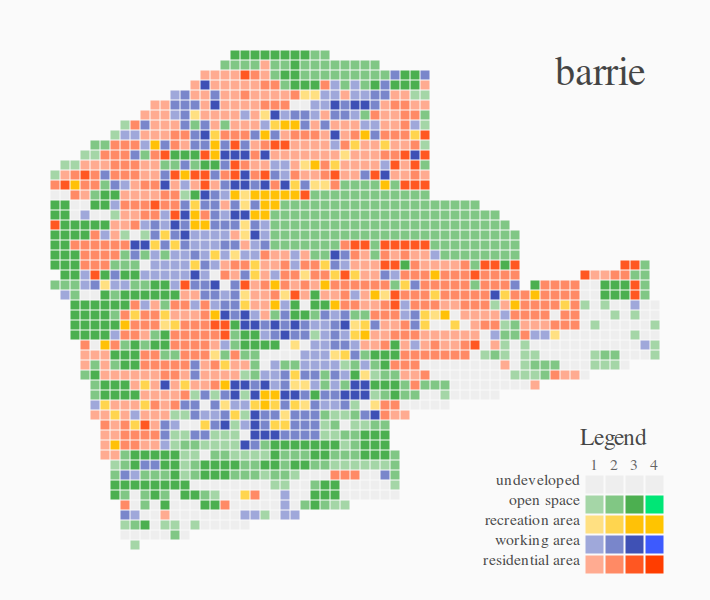
\includegraphics[width=6cm]{pic/barrie-development.png}
  }
  \subfigure[Barrie bus station]{
    \label{fig:subfigure:barrie-bus}
    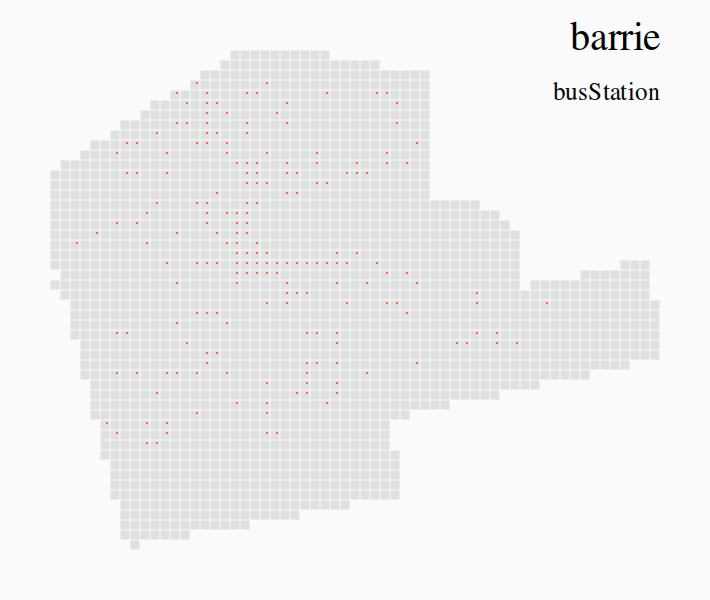
\includegraphics[width=6cm]{pic/barrie-busStation.png}
  }
  \subfigure[Nottingham development]{
    \label{fig:subfigure:nottingham-development}
    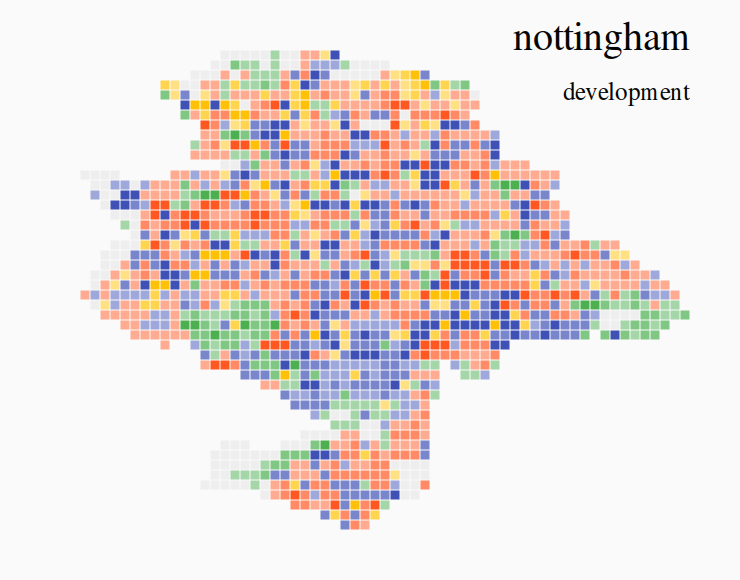
\includegraphics[width=6cm]{pic/nottingham-development.png}
  }
  \subfigure[Nottingham bus station]{
    \label{fig:subfigure:nottingham-bus}
    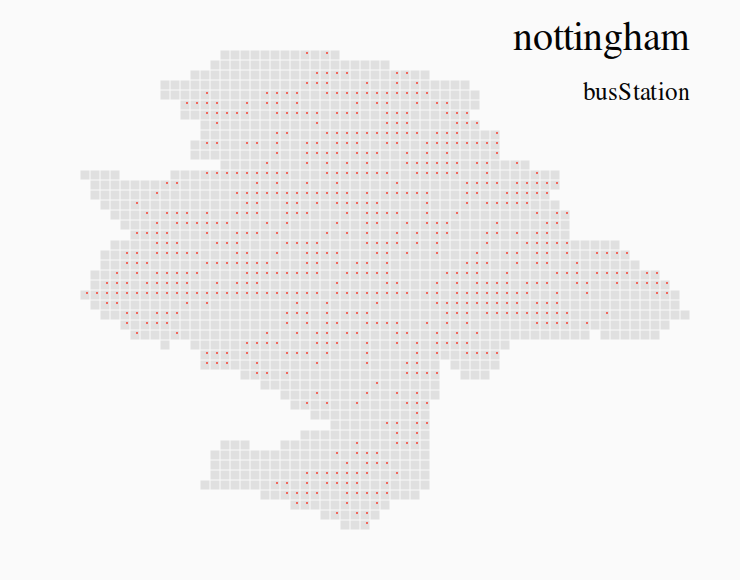
\includegraphics[width=6cm]{pic/nottingham-busStation.png}
  }
  \caption{}
\end{figure}

\subsection{Analysis of Nottingham}
\begin{table}[tb]
\centering
  \begin{tabular}{c|cccc}
    \hline
    Type & residential area & working area & recreation area & open space \\
    \hline
    Accounting for & 49.30\% & 32.07\% & 10.25\% & 13.96\% \\
    \hline
    Average level & 1.59 & 1.96 & 1.85 & 1.53 \\
    Average level*\footnote{(under government's plan)} & 1.66 & 2.28 & 2.05 & 1.53 \\
    \hline
  \end{tabular}
  \caption{Notthingham Distribution Data\footfullcite{pdf:the-nottingham-growth-plan}}
  \label{tab:nottingham-data}
\end{table}

As is shown in figure \ref{fig:subfigure:nottingham-development} \ref{fig:subfigure:nottingham-bus} and in table \ref{tab:nottingham-data}, the urban area of Nottingham city mainly consists of residential area, while open space accounts little.
It is worth noticing that working and recreational area has a relatively high development level, which is closely related to Nottingham's paying attention to technology, retail trade and advanced education.
However, it means that residential area has a lower development comparing to working area, indicating that the government's focus has long been on economic growth rather than people's happiness.
\\
\begin{table}[tb]
\centering
  \begin{tabular}{c|cccc|c}
    \hline
    Item & mix land use & beauty & residential choice & transport convenience & average \\
    \hline
    Score & 70.60 & 72.20 & 86.91 & 93.41 & 80.78 \\
    Score*\footnote{(under government's plan)} & 75.14 & 73.33 & 84.51 & 92.30 & 81.32 \\
    \hline
  \end{tabular}
  \caption{Notthingham Score under Smart Growth Metric}
  \label{tab:nottingham-score}
\end{table}
Combining data from table \ref{tab:nottingham-score} and distribution in figure \ref{fig:subfigure:nottingham-development} \ref{fig:subfigure:nottingham-bus}, we can find that working area contentrates in the middle part of the city's downtown, while residential and recreation area scatters around the downtown, which leads to a decrease in the score of mix land use.
As for the low performance in beauty, it seems contradictory to the temperate maritime climate, which is very suitable for plants to grow.
Nevertheless, if considering that Nottingham has a far more prosperous economy than the rest of Britain\footfullcite{wiki:nottingham-gdp}, it is not surprising that Notthingham, known as `a Technology City', inevitably sacrifices open space to give way to economic and technology development.
The low beauty score is against Pr.6, which emphasizes `critical environmental areas';
the convenient transport and diverse choices in residential area matches Pr.3 \& Pr.8.
\\
\begin{figure}[htb]
  \label{fig:nottingham-patch-diff}
  \centering
  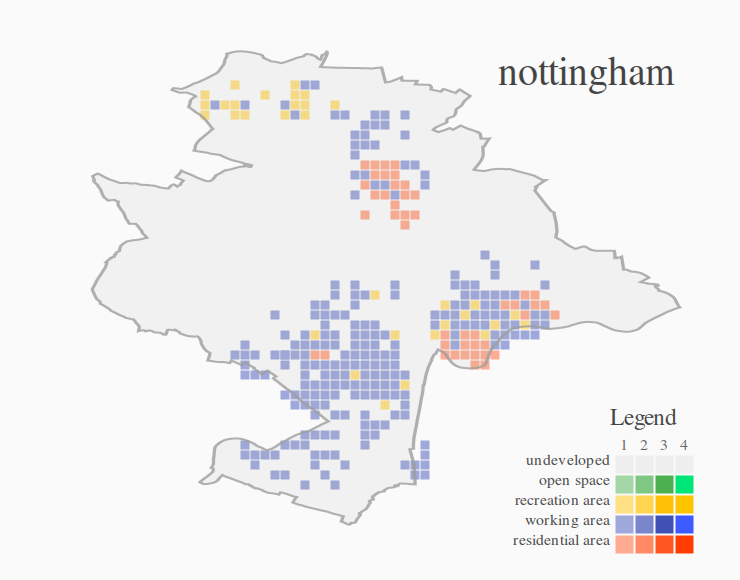
\includegraphics[width=6cm]{pic/nottingham-patch-diff-development.png}
  \caption{Nottingham development according to the government's plan}
\end{figure}
According to the government's growth plan and our smart growth metric, the city has some improvements, which is shown in figure \ref{fig:nottingham-patch-diff}.
It can be easily found that the following areas have a greater priority in the government's plan:
\begin{itemize}
  \item working area in downtown
  \item railway station neighbourhood
  \item northern residential and recreation area
\end{itemize}
To put it simple, the government still pays great attention to working area.
\\
As for the updated score under the government's plan in table \ref{tab:nottingham-data} and table \ref{tab:nottingham-score}, the residential choice score decreases due to the continuing ignorance of people's housing quality.
On the other hand, there is improvement in mix land use, for the sake of the development in the two area outside downtown.
\\
It is worth pointing out that, the growth plan we found doesn't refer to any development in open land; the file heavily depicts the techinal improvement for the city's landmarks - Boots and Biocity.
So it can be inferred that the government decides to further enhance the city's dominant industry.
The decision may meet its growth need to some extent, but it is still far from `Smart Growth Principle'.

\subsection{Analysis of Barrie}
\begin{table}[tb]
\centering
  \begin{tabular}{c|cccc}
    \hline
    Type & residential area & working area & recreation area & open space \\
    \hline
    Accounting for & 35.3\% & 20.97\% & 15.47\% & 36.30\% \\
    \hline
    Average level & 1.66 & 1.78 & 2.08 & 2.16 \\
    \hline
  \end{tabular}
  \caption{Barrie Distribution Data}
  \label{tab:barrie-data}
\end{table}

As is shown in figure \ref{fig:subfigure:barrie-development} \ref{fig:subfigure:barrie-bus} and in table \ref{tab:barrie-data}, working and recreation area has a rather small portion, while recreation area and open space develops much better than the rest.
The city of Barrie can be divided into three S-shape stripe zones: the left part is mostly residential, the middle part commercial, the right part mixing residents and recreation.
The high development of recreation area should owe to various winter-sport stadiums in the right zone, which is also a feature of city Barrie.
The heavy forest and large water area around the borderline of Barrie adds to the natural environment of the city's beauty; however, the heavy occupancy of land also forms an obstacle to the commercial development.
Comparing to Nottingham's terrian (see figure \ref{fig:subfigure:nottingham-development}), Barrie has a lower density of working area at the borderline, which may interfere with commercial communication.
\\
\begin{table}[tb]
\centering
  \begin{tabular}{c|cccc|c}
    \hline
    Item & mix land use & beauty & residential choice & transport convenience & average \\
    \hline
    Score & 54.24 & 92.11 & 64.06 & 50.67 & 65.27 \\
    Score*\footnote{(under government's plan)} & 57.93 & 92.50 & 62.73 & 57.70 & 67.72\\
    \hline
  \end{tabular}
  \caption{Barrie Score under Smart Growth Metric}
  \label{tab:barrie-score}
\end{table}
In table \ref{tab:barrie-score}, the first three scores reflects that the three `S-stipe zones' largely interrupts Barrie's adapting to `Pr.1'(mix land use) and housing choice in `Pr.3'.
It's worth mentioning that roads in Barrie are a lot wider (and the distribution is more discrete than in Nottingham), so people tenf to drive instead of taking a bus, which is contrary to diverse transport choices in `Pr.8'.
\\
We looked up for the plan of Barrie government \cite{pdf:barrie-downtown-plan} \cite{pdf:barrie-waterfront} \cite{pdf:barrie-official-plan} \cite{pdf:barrie-industrial-mapping} and arrange out the following improvements, shown in figure \ref{fig:barrie-patch-diff}.
\begin{figure}[htb]
  \label{fig:barrie-patch-diff}
  \centering
  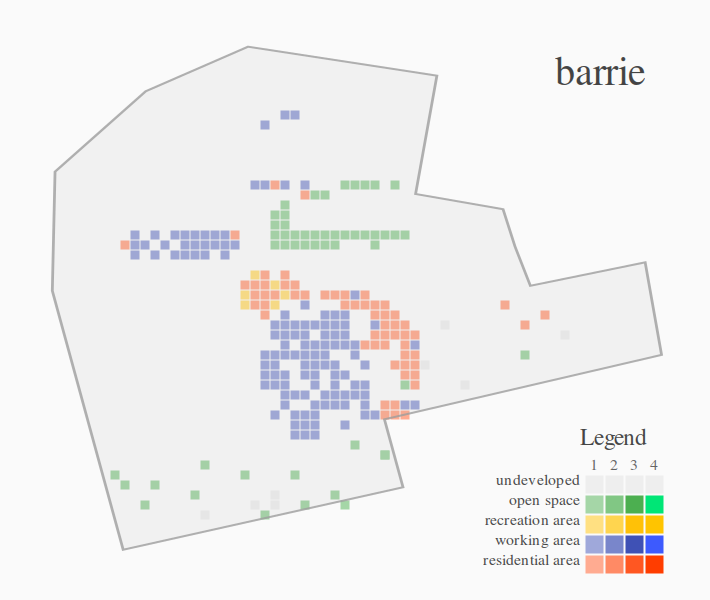
\includegraphics[width=6cm]{pic/barrie-patch-diff-development.png}
  \caption{Barrie development according to the government's plan}
\end{figure}
The government seems to have realized their ignorance in commercial, so the improvements concertrated in the mid S-stripe zone, the right stripe zone and at the same time improve the lake area.
It is obvious that the government still pays great attention to economic development, since 55.35\% efforts are made to working area.
The score under the government's plan is shown in table \ref{tab:barrie-score}.
\\
The government of Barrie seems to take a very different approach from that of Nottingham; it emphasizes its weak points rather than becoming a tourism city.
However, the S-shape stripe zones still largely interfere with the diverse development.
It is hard to make a big change in the city's functional distribution just in a short time of 10 years.

%-------------------------------------%
%-------------------------------------%
%-------------------------------------%

\section{Growth plan based on our metric}
%基于我们的metric给出的growth plan
%调控的方案是多种多样的,我们不可能考虑到所有的情况;所以我们有必要基于smart growth principles给出一定的假设,从而给出我们推荐的growth plan。
Since there are many ways to give a growth plan it's impossible for us to take all possibilities into consideration.
So we shall recommend our growth plan based on smart growth principles and certain hypothesis.
%简化假设
\subsection{Simplifying assumptions}
%根据Pr.2,应提倡compact building design,也就是应优先发展发展程度较低的地块。
\begin{itemize}
  \item According to Pr.2, we should advocate compact building design, which means we should develop square units with low development level preferentially.
%根据Pr.7,我们提倡direct development towards existing communities,这意味着不能过度地开发改建地块。所以我们认为每年在新地块开发改建上的投入不能超过总投入的20%。
  \item According to Pr.7, we should advocate direct development towards existing communities, which means we shouldn't overdevelop unused areas. So we assume investment in unused areas or redevelopment shouldn't exceed 20\% of gross investment.
%根据Pr.9,in order to make decisions cost effective,我们在选取最优growth plan时选用使得综合得分提升最高的方案。
  \item According to Pr.9, in order to make decisions cost effective, we will choose the growth plan which results in maximum overall score increment.
%根据Pr.10,我们应该根据各个分区的需要重新对投入进行分配,调整在不同区域类型上的投入比例。
  \item According to Pr.10, we will distribute our investment into different types of areas and adjust investment proportions.
%我们给出的growth plan的总投入与之前调查到的政府给予的总投入是相同的。
  \item Our growth plan will use same amout of investment as the government based on previous research.
%使得每个square unit的发展程度增加1的投入是相同的。
  \item We assume we will always invest the same to make a square unit development level increase one.
%由于所调查到的政府growth plan都是约10年的发展计划,所以我们每隔10年给出一个growth plan,共给出30年的growth plan。
  \item Since government growth plans are both 10-year development plan, we will make a growth plan every 10 year and together three consecutive plans make a 30-year growth plan.
%发展后所有square unit的发展程度不超过4。
  \item We assume no square unit's development level will exceed 4.
%我们只对unused area和发展程度为1的open space(一般是farmland)进行开发改建。
  \item We will only redevelop open space area with 1 development(generally farmland).
\end{itemize}

%发展意愿函数
\subsection{Development will function}
%容易发现,对于【G3】,由于其发展意愿和【G8】以及投入分别反相关,所以【G3】对于发展程度加t的意愿指数为【G26】。我们每次将选择一个意愿指数最高的square unit及其对应的t,对其进行t的投入,随后将整个地图更新后重新计算每个square unit。
It's easy to see that, as for $ A_{ij} $, since its development will is negative correlated with $ d_{ij} $, $ A_{ij} $'s develop will when we add t to its development level is $$ w(i,j)=\frac{\Delta (G_m+G_b+G_h)}{t\cdot d_{ij}}=\frac{f_{r_m, k_m}^{'} (M) \cdot \Delta M + f_{r_b, k_b}^{'} (B) \cdot \Delta B + \Delta G_h}{t \cdot d_{ij}}. $$ So, we choose a square unit with the highest develop will point along with its $t$, add $t$ to its development level, and upgrade the whole map and recalculate every square unit's will point.
\\
%当然这里也可以假设线性叠加,直接挑选意愿指数最高的若干个。但是我们并没有这样做。
Of course we can assume the function is linear, and directly choose several square units with highest development will points, but we still choose to upgrade the map after each choice.
%这事实上也是一种贪心法的实现。
This actually is another type of greedy method.

%Nottingham的growthplan
\subsection{Nottingham's growth plan}
%以下是每隔十年给出的growth plan。【P5】
The following is Nottingham's growth plan (every 10 years).[P5]
%以下是三十年后的城市分区情况与现在的城市分区情况对比。【P6】
The following is a comparison in city's square units between 30 years later and present.[P6]
%以下是新增公交站点的情况。【P7】
The following is newly added bus stations' distribution. [P7]
%对于第一个十年growth plan,综合得分为67.72分,分布多样性得分、景观得分、住房选择自由和交通便捷得分依次为57.93分、92.50分、62.73分、57.70分。可以发现,我们的计划中将46.39%的投入花在了open space的建设上,而对于其余三个区域类别的投入较为平均。住房选择自由的得分相比政府的growth plan有了显著的提升,可以被理解成第一个10年的growth plan没有显著特点的原因。因为可以看出,第二个10年的growth plan主要是发展了downtown部分的自然景观(因为downtown部分高速发展科技的过程中势必使得此地区的open space匮乏)和高纬度地区的working area(那里主要四散着residential area和recreation area);而第三个10年时由于自然景观的弱势已经被逐渐削减,所以开始在高纬度地区逐渐发展原本的优势分区working area和recreation area(downtown部分较为发达,所以不优先发展,这遵循了Pr.2)。第一个十年分布没有特点的原因就是弥补了部分地区住房选择不够匹配的缺陷,其次是大力发展自然景观后在其他分区的投入会稍显不足。
As for the first 10-year growth plan, we obtain 67.72 points in overall score. The growth plan scores 57.93 points, 92.50 points, 62.73 points and 57.70 points in mix land use, beauty, housing and transportation. We can discover that in this plan, it spends 46.39\% invesment on open space development, and relatively average investment on other three types of areas. Housing score increases remarkably compared to government's growth plan, which can be interpreted as the reason for the plan's lack of prominent characteristic. In the second 10-year growth plan, it mainly develops open spaces in the downtown (open spaces are scarce in the downtown due to its major focus on hi-tech development) and working areas in the north part of the city (residential areas and recreational areas are distributed there). In the third 10-year growth plan, since the city's beauty score has increased a lot, it begins to develop working areas and recreational areas in the north part of the city. (Downtown is more developed, so it's not our priority according to Pr.2) The reason for the first 10-year growth plan's irregularity is to improve low housing conditions in certain areas in the city. Next, it focuses on development in open spaces, and less focused on other areas.
%对于30年的规划,我们对于residential area、working area、recreational area、open space以及undeveloped的投入比例分别为6.45%,23.94%,13.24%,44.14%,11.88%。也就说如果按发展潜力从高到低排序的话,Nottingham依次应该发展open space,working area,recreation area,undeveloped area和residential area。发展open space是因为smart growth principle中明确提及了自然景观的建设需求,而这恰恰又是Nottingham作为“科技之城”最为匮乏的一点。而发展working area正是Nottingham的growth need(这从政府的决策可以看出),这也恰恰证明了smart growth principles虽然并不与growth need相符,但绝不是背道而驰。smart growth principles本质上是在让城市更均衡地发展的同时遵循自身的growth need而继续发展。
In the 30-year growth plan, we invest 6.45\%, 23.94\%, 13.24\%, 44.14\% and 11.88\% of total investment respectively on residential areas, working areas, recreational areas, open spaces and undeveloped areas. It suggests that if we rank different types of areas in Nottingham from the most potential to the least potential, it would be open space,working area,recreational area,undeveloped area and residential area. Developing open spaces is to meet the need of vast natural landscape mentioned in smart growth principles, which is also the weakness of the 'technology city' Nottingham. Developing working area is also Nottingham's growth need, which can be interpreted from the government's plan, which suggests that smart growth principles may not entirely correlate with a city's growth need, but definitely do not contradict with it. So in essence, smart growth principles are designed to make a city grow in a more balanced way, and meet the city's need at the same time.
%三十年的growth plan中也存在着一定的不足之处。由于open space分布太少,所以围绕downtown的诸多open space的发展程度到了4。这与现实情况是不符的;这意味着在真实的城市growth plan中,是需要对分区规划进行改动来加以平衡downtown地区的open space需求的。
The 30-year growth plan also have its disadvantages. Due to lack of open spaces, many open spaces downtown are developed into level 4, which is not realistic. It means in a real city growth plan, we need to adjust investment in different areas to balance the need of open space in the downtown.

%Barrie的growthplan
\subsection{Barrie's growth plan}
%以下是每隔十年给出的growth plan。【P8】
The following is Barrie's growth plan (every 10 years).[P8]
%以下是三十年后的城市分区情况与现在的城市分区情况对比。【P9】
The following is a comparison in city's square units between 30 years later and present.[P9]
%以下是新增公交站点的情况。【P10】
The following is newly added bus stations' distribution.[P10]
%对于第一个十年growth plan,综合得分为78.55分,分布多样性得分、景观得分、住房选择自由和交通便捷得分依次为65.88分、92.02分、89.42分、66.89分。容易发现,之前极为弱势的分布多样性得分和住房选择性得分瞬间得到了增长;这是因为在左边的大多是residential area的带状区域中建设了working area,而在中间的大多是working area的带状区域中建设了residential area,打破了之前的三个带状区域的僵局。同样道理地,第二个十年着重于打破左右两个带状区域的单一布局(因为Barrie的residential area分布较广,发展压力较小),第三个十年中为了弥补第二个十年所放弃的residential area的发展,开始着重于在中间带状区域中增加residential area的分布和低纬度的边界区working area分布(因为那个区块大多是residential area)。
The first 10-year growth plan scores 78.55 points overall. The growth plan scores 65.88 points, 92.02 points, 89.42 points and 66.89 points in mix land use, beauty, housing and transportaion. It's obvious that mix-land-use and housing score increase tremendously, which is because that working areas are developed in the left side of S-shape stripe zone, where most of the square units are residential areas, and residential areas are developed in the center of S-shape stripe zone, where most of the square units are working areas. After development in this growth plan, three distinct S-shape strip zone no longer exists. In the second 10-year plan, it also focuses on eliminate flat distribution of squares in the S-stripe areas in the west and east side. Because Barrie's residential areas are well-distributed, their development is not our priority. However, in the third 10-year growth plan, in order to make up the ignorance of residential areas in the previous 10 years, it starts to develop residential areas in the middle S-stripe shape area and working areas in the south part (Most areas there are residential squares).
%对于30年的规划,我们对于residential area、working area、recreation area、open space以及undeveloped的投入比例分别为24.45%,32.94%,31.41%,0,16.30%。对比政府政策为residential area、working area、recreation area分别投入26.05%,55.35%,2.79%,我们可以看出对待residential area的态度是相近的,但政府对于recreation area的建设较为忽略。这是不满足Pr.1的。按发展潜力从高到低排序的话,Barrie依次应该发展working area,recreation area,residential area,undeveloped area和open space。由于Barrie的open space条件实在优异,而working area明显不足,所以优先发展working area而暂时不发展open space。
In the 30-year growth plan, we invest 24.45\%, 32.94\%, 31.41\%, 0\% and 16.30\% of total investment respectively on residential areas, working areas, recreation areas, open spaces and undeveloped areas. Compared to government's plan which invest 26.05\%, 55.35\% and 2.79\% respectively on residential areas, working areas and recreational areas, we can see that both plans treat residential areas similarly, but the goverment overlooks investment on recreational areas. It doesn't meet Pr.1. So if we rank different types of areas from most potential to least potential, it would be working area, recreational area, residential area, undeveloped area and open space. Since Barrie does own a lot of open spaces but lack working areas, it seems reasonable for Barrie to develop working areas first and put open space development aside.
%对比nottingham的五个区域类型的发展潜力,我们可以发现除去对open space的需求明显不同外,其余的几个区域类型发展潜力大小近乎类似。只是因为两个城市的residential area都占了城市的较大比重,暂时不需要承载人口快速增长的压力,所以相比发展另两个区域类型显得不那么重要。但是他们发展working area虽然都是为了顺应自身的growth need,但原因是截然不同的,Nottingham是为了扩大优势,而Barrie是为了弥补劣势。
\subsection{summary}
Compared with Nottingham's development potential in five different types of areas, we can find that despite Barrie and Nottingham have entirely different need for open space, but any other type's development potential is quite close. Because both cities' residential parts take up most of their areas, they don't have to face high population growth pressure. So it seems less important to develop residential areas compared with working and recreational areas. Although they both develop working areas to meet their own growth need, their starting point is divergent. Nottingham develop working areas to strengthen its advantages, but Barrie is to make up for its weakness.

\printbibliography

%-------------------------------------%
%-------------------------------------%
%-------------------------------------%


\end{document}
